\begin{frame}

\begin{center}
  \huge Procediamo con il nostro primo \\
  \huge Hello World! 
\end{center}

\end{frame}

\subsection{Hello World}
\begin{frame}[fragile]

\frametitle{Primo Hello World}
 
 Nel file principale (che per semplicità chiamiamo \texttt{main.tex}) inseriamo 
il seguente codice:

\begin{lstlisting}[frame = single, title={File main.tex}] 
\documentclass{beamer}
\usepackage[utf8]{inputenc}

\usepackage{../UnipdTheme/Padova/beamerthemePadova}
\usepackage{listings}
\usepackage{amsmath, amssymb}
\usepackage{xcolor}
\usepackage{listingsutf8}
\lstset{language = Tex}

\usepackage[absolute,overlay]{textpos}


\author{Davide Polonio}
\date{27/07/2017}
\title{Primo progetto di Prova}

\begin{document}

\maketitle

\input{res/listOfSections}
\end{document}
 
\end{lstlisting}

\end{frame}

\begin{frame}[fragile]
 
 \frametitle{Aggiungiamo codice...}
 
 Creiamo altri file
 
 \begin{lstlisting}[frame = single, title={File res/config/package.tex}]
\documentclass[12pt]{book}

\usepackage{graphicx}
\usepackage{float}
 \end{lstlisting}

 e...
 
 \begin{lstlisting}[frame = single, title={File res/listOfSections.tex}]
\input{res/sections/parte1}
 \end{lstlisting}

Nota: negli input non è necessario inserire l'estensione dei file! 
\end{frame}

\begin{frame}[fragile]
 
 \frametitle{Contenuto, finalmente!}
 
 Finalmente aggiungiamo il contenuto che vogliamo
 
 \begin{lstlisting}[frame = single, title={File res/sections/parte1.tex}]
\textit{Ciao mondo!}
 \end{lstlisting}
 
 Aggiungiamoci anche un'immagine!
 Copiamola in \texttt{res/img/} rinominiamola con il nome \texttt{immagine}. 
Ora aggiungiamo il seguente codice al file \texttt{parte1.tex}

 \begin{lstlisting}[frame = single]
\begin{figure}[h!]
 \centering
 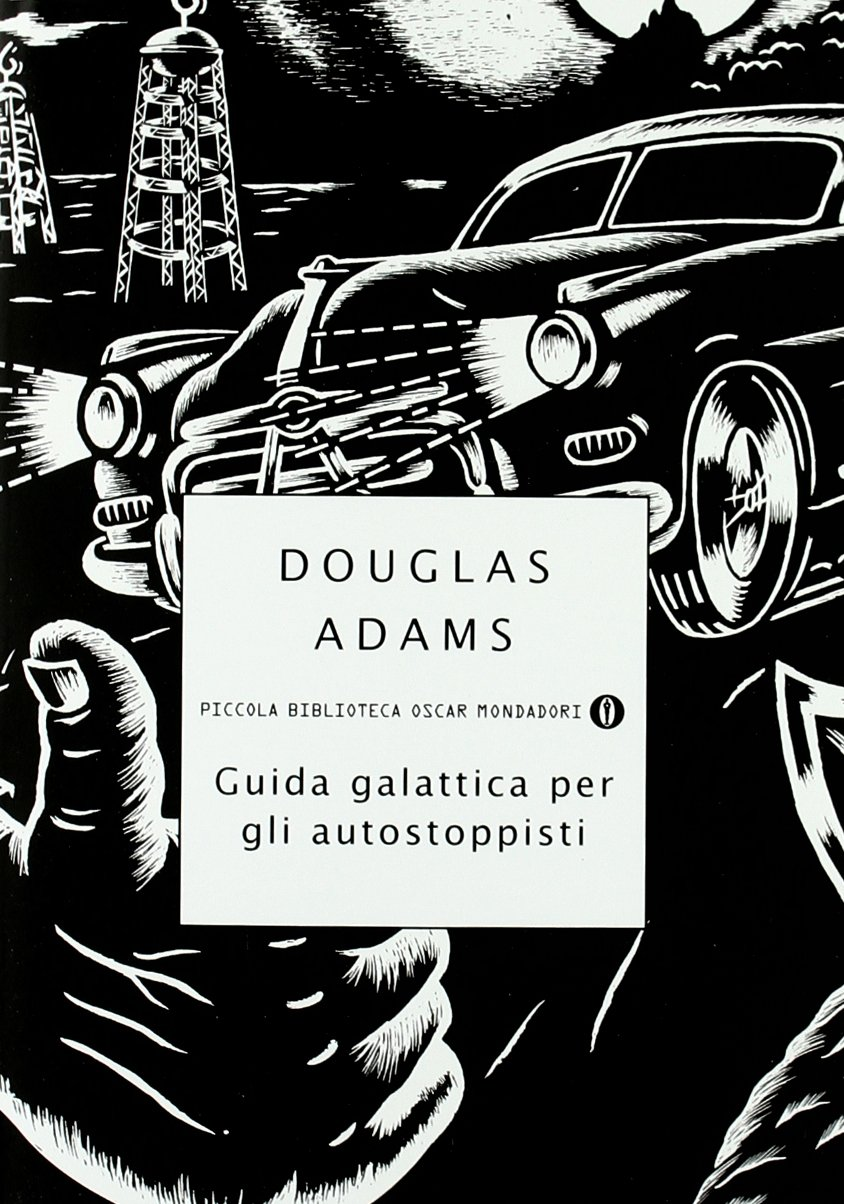
\includegraphics[scale=0.5]{res/img/immagine}
 \caption{Una immagine bellissima.}
\end{figure}
 \end{lstlisting}


\end{frame}

\begin{frame}
 \frametitle{Ora il passo finale...}
 
 \huge Compiliamo!
 
 
 \begin{textblock*}{5cm}(6.5cm,3cm)
   
\includegraphics[scale=0.5]{icon-build}
 \end{textblock*}
\end{frame}
